\chapter{Multiplets de moment cinétique, mouvement radial et échelle de l’oscillateur}

\section{Dépendance angulaire de la fonction d’onde}

Une particule dans un champ de force central possède une coordonnée radiale et deux coordonnées angulaires. En mécanique classique,
\begin{equation}
\mathbf L=\mathbf r\times\mathbf p
\end{equation}
est conservé en tant que vecteur. Sa direction fixe le plan de l’orbite, qui n’est pas nécessairement circulaire.

En mécanique quantique, la particule est décrite par
\begin{equation}
\Psi=\Psi(r,\theta,\phi),
\end{equation}
et le moment cinétique concerne la dépendance de cette fonction d’onde par rapport aux angles.

Dans un espace à deux dimensions, il n’existe qu’une seule composante du moment cinétique, génératrice des rotations autour de l’axe perpendiculaire au plan :
\begin{equation}
L_z=-i\hbar\frac{\partial}{\partial\theta}.
\end{equation}
Une fonction propre de valeur propre \(\hbar\ell\) vérifie
\begin{equation}
-i\hbar\frac{\partial}{\partial\theta}\psi(r,\theta)
=\hbar\ell\,\psi(r,\theta).
\end{equation}
La coordonnée \(r\) est un paramètre spectateur dans cette équation. Sa solution est de la forme
\begin{equation}
\psi(r,\theta)=\chi(r)e^{i\ell\theta}.
\end{equation}
Pour une fonction d’onde orbitale ordinaire, monovaluée, le retour au même point après \(\theta\to\theta+2\pi\) impose que \(\ell\) soit un entier. Le facteur radial \(\chi(r)\) peut influer sur l’énergie, mais pas sur cette valeur propre du moment cinétique.

L’analogue tridimensionnel sépare la dépendance radiale des fonctions définies sur la sphère :
\begin{equation}
\Psi(r,\theta,\phi)=R(r)Y_{\ell m}(\theta,\phi).
\end{equation}
Les fonctions \(Y_{\ell m}\) sont les harmoniques sphériques. Il ne sera pas nécessaire d’en connaître les expressions explicites ici. Les rotations agissent sur le facteur angulaire, tandis que la fonction radiale reste inchangée.

\section{Multiplets finis de moment cinétique}

Les composantes du moment cinétique vérifient
\begin{equation}
\begin{aligned}
[L_x,L_y]&=i\hbar L_z,\\
[L_y,L_z]&=i\hbar L_x,\\
[L_z,L_x]&=i\hbar L_y.
\end{aligned}
\end{equation}
Choisissons des états propres de \(L_z\),
\begin{equation}
L_z|\ell,m\rangle=\hbar m\,|\ell,m\rangle,
\end{equation}
et définissons
\begin{equation}
L_\pm=L_x\pm iL_y.
\end{equation}
Les commutateurs
\begin{equation}
[L_z,L_\pm]=\pm\hbar L_\pm
\end{equation}
donnent
\begin{align}
L_z\bigl(L_\pm|\ell,m\rangle\bigr)
&=\bigl(L_\pm L_z+[L_z,L_\pm]\bigr)|\ell,m\rangle \\
&=\hbar(m\pm1)L_\pm|\ell,m\rangle.
\end{align}
Ainsi, \(L_+\) augmente \(m\) d’une unité et \(L_-\) le diminue d’une unité, sauf si le vecteur obtenu est nul.

Un multiplet fini possède un état de plus haut poids et un état de plus bas poids :
\begin{equation}
L_+|\ell,\ell\rangle=0,
\qquad
L_-|\ell,-\ell\rangle=0.
\end{equation}
Les directions \(+z\) et \(-z\) sont reliées par une rotation ; le spectre fini est donc symétrique par rapport à zéro. Ses valeurs sont donc
\begin{equation}
m=-\ell,-\ell+1,\ldots,\ell-1,\ell,
\end{equation}
et le nombre d’états est
\begin{equation}
2\ell+1.
\end{equation}
Comme deux valeurs voisines diffèrent d’une unité, les extrémités peuvent être des entiers ou des demi-entiers. Les harmoniques sphériques orbitales ordinaires réalisent le cas entier ; l’algèbre abstraite du moment cinétique admet aussi des multiplets demi-entiers.

\begin{classroomqa}\lecturetimestamp{00:16:12}\audiencequestion{Un multiplet de moment cinétique peut-il contenir un nombre infini d’états ?}\lecturerresponse{On peut envisager cette possibilité, mais elle ne sera pas nécessaire ici. En général, le moment cinétique augmente l’énergie lorsque les autres caractéristiques de l’état sont maintenues fixes ; les états de moment cinétique infini ne sont donc pas pertinents lorsqu’on étudie les états d’énergie finie.}\end{classroomqa}

\section{La valeur commune de \texorpdfstring{\(L^2\)}{L au carré}}

L’opérateur qui mesure le carré de la norme du moment cinétique est
\begin{equation}
L^2=L_x^2+L_y^2+L_z^2.
\end{equation}
Le produit ordonné des opérateurs d’échelle est
\begin{align}
L_-L_+
&=(L_x-iL_y)(L_x+iL_y) \\
&=L_x^2+L_y^2+i[L_x,L_y] \\
&=L_x^2+L_y^2-\hbar L_z.
\end{align}
Par conséquent,
\begin{equation}
L^2=L_z^2+\hbar L_z+L_-L_+.
\end{equation}
Appliquons cette identité à l’état de plus haut poids. Puisque \(L_+|\ell,\ell\rangle=0\),
\begin{align}
L^2|\ell,\ell\rangle
&=\left(L_z^2+\hbar L_z+L_-L_+\right)|\ell,\ell\rangle \\
&=\hbar^2\left(\ell^2+\ell\right)|\ell,\ell\rangle,
\end{align}
et donc
\begin{equation}
L^2|\ell,\ell\rangle
=\hbar^2\ell(\ell+1)|\ell,\ell\rangle.
\end{equation}
Le carré de la norme n’est pas \(\hbar^2\ell^2\). Le terme supplémentaire découle de la non-commutativité des composantes du moment cinétique.

Cette même valeur est celle de tous les états du multiplet, et pas seulement de l’état de plus haut poids.

\begin{classroomqa}\lecturetimestamp{00:26:08}\audiencequestion{Que montre exactement l’exercice qui établit que les autres états ont la même valeur de \(L^2\) ?}\lecturerresponse{Montrez que \(L^2\) commute avec chaque composante du moment cinétique, et donc avec \(L_-\). Faites ensuite commuter \(L^2\) à travers \(L_-\) : si l’état de plus haut poids a pour valeur propre \(\hbar^2\ell(\ell+1)\), l’état suivant dans l’échelle a la même valeur propre. En répétant le raisonnement, on retrouve cette valeur tout au long de l’échelle.}\end{classroomqa}

En effet,
\begin{equation}
[L^2,L_i]=0,
\qquad i=x,y,z,
\end{equation}
donc
\begin{equation}
[L^2,L_\pm]=0.
\end{equation}
Par exemple,
\begin{align}
L^2\bigl(L_-|\ell,\ell\rangle\bigr)
&=L_-L^2|\ell,\ell\rangle \\
&=\hbar^2\ell(\ell+1)L_-|\ell,\ell\rangle.
\end{align}
En poursuivant vers le bas, on obtient
\begin{equation}
L^2|\ell,m\rangle
=\hbar^2\ell(\ell+1)|\ell,m\rangle
\end{equation}
pour tout \(m=-\ell,\ldots,\ell\).

L’ordre inverse donne une factorisation équivalente :
\begin{align}
L_+L_-
&=(L_x+iL_y)(L_x-iL_y) \\
&=L_x^2+L_y^2-i[L_x,L_y] \\
&=L_x^2+L_y^2+\hbar L_z,
\end{align}
et par conséquent
\begin{equation}
L^2=L_z^2-\hbar L_z+L_+L_-.
\end{equation}

\begin{classroomqa}\lecturetimestamp{00:32:05}\audiencequestion{Peut-on factoriser \(L_x^2+L_y^2\) dans l’ordre inverse en utilisant \(L_+L_-\) ?}\lecturerresponse{Oui. Le signe du terme en \(L_z\) s’inverse. Avec cet ordre, on applique l’identité à l’état de plus bas poids, annulé par \(L_-\), plutôt qu’à l’état de plus haut poids. On retrouve la même valeur propre \(\hbar^2\ell(\ell+1)\).}\end{classroomqa}

Les harmoniques sphériques vérifient donc
\begin{align}
L^2Y_{\ell m}
&=\hbar^2\ell(\ell+1)Y_{\ell m}, \\
L_zY_{\ell m}
&=\hbar m\,Y_{\ell m}.
\end{align}
Pour chaque valeur orbitale \(\ell=0,1,2,\ldots\), il existe \(2\ell+1\) fonctions, indexées par \(m=-\ell,\ldots,\ell\).

Pour un potentiel central,
\begin{equation}
[H,L_i]=0.
\end{equation}
Lorsqu’on fixe un état propre radial de l’énergie et \(\ell\), modifier \(m\) au moyen de \(L_\pm\) ne change pas l’énergie. Chaque état propre radial engendre donc un multiplet magnétique de dimension \(2\ell+1\).

L’échelle orbitale entière est représentée ci-dessous.\footnote{Le diagramme est reconstitué à partir du schéma du multiplet et des identités d’opérateurs visibles à \(00{:}35{:}53\) de la vidéo du cours.}

\begin{figure}[htbp]\centering
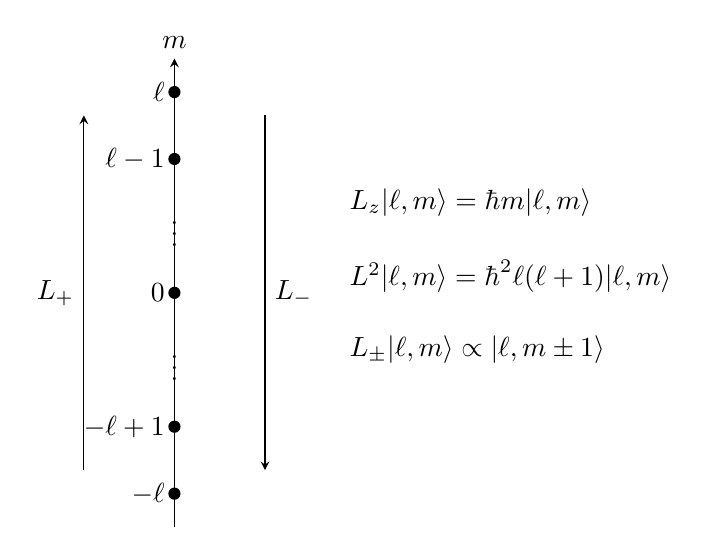
\begin{tikzpicture}[x=1cm,y=0.85cm,>=stealth]
\draw[->] (0,-3.5) -- (0,3.5) node[above] {$m$};

\fill (0,3) circle (2.2pt);
\fill (0,2) circle (2.2pt);
\fill (0,0) circle (2.2pt);
\fill (0,-2) circle (2.2pt);
\fill (0,-3) circle (2.2pt);

\node[left] at (0,3) {$\ell$};
\node[left] at (0,2) {$\ell-1$};
\node[left] at (0,0) {$0$};
\node[left] at (0,-2) {$-\ell+1$};
\node[left] at (0,-3) {$-\ell$};

\node at (0,1) {$\vdots$};
\node at (0,-1) {$\vdots$};

\draw[->] (-1.15,-2.65) -- (-1.15,2.65)
node[midway,left] {$L_+$};
\draw[->] (1.15,2.65) -- (1.15,-2.65)
node[midway,right] {$L_-$};

\node[anchor=west] at (2.1,1.35)
{$L_z|\ell,m\rangle=\hbar m|\ell,m\rangle$};
\node[anchor=west] at (2.1,0.25)
{$L^2|\ell,m\rangle=\hbar^2\ell(\ell+1)|\ell,m\rangle$};
\node[anchor=west] at (2.1,-0.85)
{$L_\pm|\ell,m\rangle\propto|\ell,m\pm1\rangle$};
\end{tikzpicture}\caption{Un multiplet entier de moment cinétique orbital. \(L_+\) et \(L_-\) font varier \(m\) d’une unité, tandis que \(L^2\) reste égal à \(\hbar^2\ell(\ell+1)\) dans tout le multiplet.}\lectureframe{00:35:53}\end{figure}

\section{Le problème des forces centrales}

Considérons
\begin{equation}
H=\frac{\mathbf p^2}{2m}+V(r),
\end{equation}
où \(V\) ne dépend que de la distance à l’origine. La symétrie de rotation implique la conservation du moment cinétique. En mécanique classique, \(\mathbf L\) conserve une norme et une direction fixes, de sorte que l’orbite reste dans un plan perpendiculaire à \(\mathbf L\). L’orbite n’est pas nécessairement circulaire, ni même fermée.

Choisissons les coordonnées de sorte que ce plan orbital classique soit le plan \(xy\), et décomposons la quantité de mouvement en composantes radiale et tangentielle :
\begin{equation}
\mathbf p^2=p_r^2+p_\theta^2.
\end{equation}
Puisque la norme du moment cinétique est
\begin{equation}
L=r p_\theta,
\end{equation}
la contribution tangentielle s’écrit
\begin{equation}
p_\theta^2=\frac{L^2}{r^2}.
\end{equation}
Le Hamiltonien devient
\begin{equation}
H=\frac{p_r^2}{2m}+\frac{L^2}{2mr^2}+V(r).
\end{equation}
À \(L\) fixé, il s’agit d’un problème unidimensionnel pour la coordonnée radiale, avec le potentiel effectif
\begin{equation}
V_{\mathrm{eff}}(r)=\frac{L^2}{2mr^2}+V(r).
\end{equation}
Le Hamiltonien radial est représenté au tableau ci-dessous.\footnote{Image source : \texttt{\detokenize{lecture_03_frame_02.png}}, vidéo du cours à \(00{:}47{:}15\).}

\begin{figure}[htbp]\centering
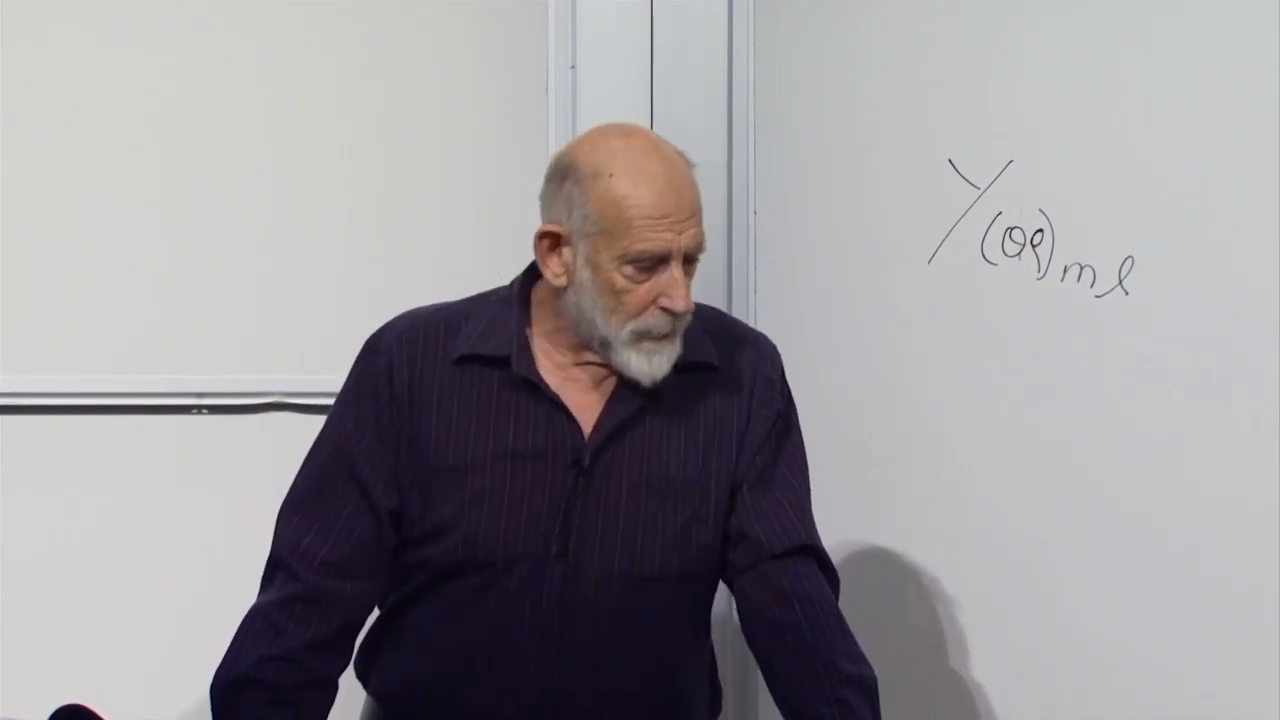
\includegraphics[width=0.9\linewidth]{lecture_03_frame_02.png}\caption{À moment cinétique classique fixé, le Hamiltonien radial comprend l’énergie cinétique radiale, le terme centrifuge \(L^2/(2mr^2)\) et le potentiel central \(V(r)\).}\lectureframe{00:47:15}\end{figure}

Le terme \(1/r^2\) constitue la barrière centrifuge. Il augmente à mesure que la particule s’approche de l’origine ; la force associée est donc dirigée vers l’extérieur. Pour les potentiels attractifs de type coulombien considérés ici, une trajectoire avec \(L\neq0\) contourne le centre au lieu de l’atteindre. Lorsque \(L=0\), la barrière disparaît.

Pour le potentiel coulombien attractif,
\begin{equation}
V(r)=-\frac{\kappa}{r},
\end{equation}
le terme centrifuge domine aux petites valeurs de \(r\), tandis que le terme coulombien décroît moins vite et domine aux grandes valeurs de \(r\). Pour \(L\neq0\), leur somme présente un minimum. Au minimum, le mouvement se fait à rayon constant et est donc circulaire. Au-dessus du minimum et en dessous du seuil d’échappement, le mouvement lié oscille entre un rayon minimal et un rayon maximal ; dans le problème coulombien, ces oscillations radiales correspondent aux oscillations d’une orbite elliptique.

\section{L’équation radiale réduite}

En mécanique quantique, la partie angulaire d’un état de moment cinétique orbital bien défini est une harmonique sphérique. Écrivons l’état séparé sous la forme
\begin{equation}
\Psi_{n_r\ell m}(r,\theta,\phi)
=\frac{u_{n_r\ell}(r)}{r}\,
Y_{\ell m}(\theta,\phi).
\end{equation}
L’opérateur angulaire \(L^2\) a pour valeur propre
\begin{equation}
L^2Y_{\ell m}
=\hbar^2\ell(\ell+1)Y_{\ell m}.
\end{equation}
Pour une paire fixée \(n_r,\ell\), abrégeons \(u_{n_r\ell}(r)\) en \(u(r)\). Il reste à résoudre pour la fonction radiale réduite l’équation
\begin{equation}
\begin{aligned}
&-\frac{\hbar^2}{2m}\frac{d^2u}{dr^2}
+\frac{\hbar^2\ell(\ell+1)}{2mr^2}u(r)\\
&\qquad+V(r)u(r)=E_{n_r\ell}\,u(r).
\end{aligned}
\end{equation}

\editorialnote{L’équation purement unidimensionnelle faisant intervenir la dérivée seconde s’écrit pour la fonction radiale réduite \(u=rR\). Ainsi, le \(\psi(r)\) dans l’équation affichée pendant le cours correspond à \(u(r)\), tandis que le facteur radial ordinaire dans \(\Psi=R(r)Y_{\ell m}\) est \(R=u/r\). Cette convention évite de traiter \(-i\hbar\,d/dr\) comme un opérateur autonome de quantité de mouvement radiale hermitien sur l’espace de Hilbert radial tridimensionnel.}

L’équation radiale réduite est représentée au tableau ci-dessous.\footnote{Image source : \texttt{\detokenize{lecture_03_frame_03.png}}, vidéo du cours à \(00{:}54{:}32\).}

\begin{figure}[htbp]\centering
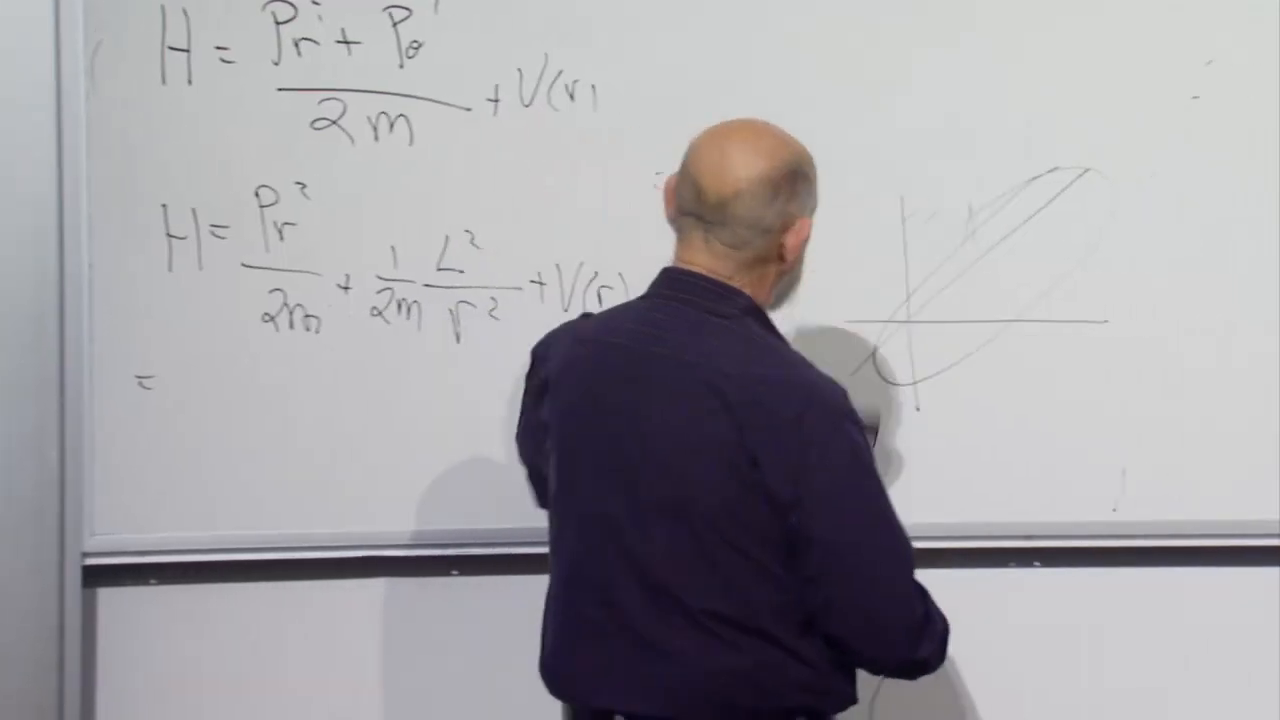
\includegraphics[width=0.9\linewidth]{lecture_03_frame_03.png}\caption{À \(\ell\) fixé, la fonction d’onde radiale réduite vérifie une équation de Schr\"odinger unidimensionnelle, avec un terme centrifuge proportionnel à \(\ell(\ell+1)/r^2\).}\lectureframe{00:54:32}\end{figure}

La structure angulaire tridimensionnelle est condensée dans le paramètre \(\ell\). Le nombre quantique magnétique \(m\) n’intervient pas dans l’équation radiale.

\begin{classroomqa}\lecturetimestamp{00:55:34}\audiencequestion{Pour une valeur donnée de \(\ell\), les \(2\ell+1\) états magnétiques ont-ils la même énergie ?}\lecturerresponse{Oui, à condition de fixer aussi l’état propre radial. Pour chaque valeur choisie de \(u_{n_r\ell}\), toutes les valeurs \(m=-\ell,\ldots,\ell\) ont la même énergie, car \(m\) n’intervient pas dans l’équation radiale. En général, des états propres radiaux différents associés à la même valeur de \(\ell\) ont des énergies différentes.}\end{classroomqa}

\begin{classroomqa}\lecturetimestamp{00:56:03}\audiencequestion{Pourquoi peut-on remplacer \(L^2\) par \(\hbar^2\ell(\ell+1)\), et quel est le lien entre \(\ell\) et les valeurs permises de \(m\) ?}\lecturerresponse{Le nombre \(\ell\) indexe un multiplet de moment cinétique et en est la plus grande valeur de \(m\). Tous les états de ce multiplet ont la même valeur propre de \(L^2\), soit \(\hbar^2\ell(\ell+1)\) ; c’est donc cette valeur propre que l’on introduit dans l’équation radiale.}\end{classroomqa}

Il n’est pas nécessaire de connaître les solutions explicites en fonctions spéciales pour l’argument présenté ici. Ce qui importe, c’est la façon dont les solutions s’organisent.

\section{Nœuds radiaux et niveaux d’énergie}

À \(\ell\) fixé, l’équation radiale réduite est un problème aux valeurs propres ordinaire à une dimension. Ses états liés se classent selon leur nombre de nœuds intérieurs. L’état radial le plus bas n’a aucun nœud intérieur, le suivant en a un, et celui d’après en a deux. Un plus grand nombre de nœuds signifie que la fonction d’onde varie plus rapidement ; une variation plus rapide implique une quantité de mouvement plus grande et donc une énergie cinétique plus élevée.

Chaque valeur de \(\ell\) définit un opérateur radial différent, car le terme centrifuge varie avec \(\ell\). Les valeurs \(\ell=0,1,2,\ldots\) donnent donc des suites radiales distinctes. Le terme centrifuge positif décale les niveaux vers le haut lorsque le moment cinétique augmente. Chaque valeur propre radiale à \(\ell\) fixé est associée à un multiplet magnétique de dimension
\begin{equation}
2\ell+1.
\end{equation}
Les niveaux \(\ell=0\) sont des singulets, les niveaux \(\ell=1\) des triplets et les niveaux \(\ell=2\) des quintuplets. Ce sont les dégénérescences imposées par la symétrie de rotation ; une symétrie supplémentaire peut aussi rendre dégénérés des états de valeurs différentes de \(\ell\).

Pour les potentiels de type atomique qui vérifient \(V(r)\to0\) aux grandes valeurs de \(r\), le seuil d’échappement est conventionnellement fixé à \(E=0\). Les états d’énergie négative forment le spectre discret des états liés. À \(E=0\) et au-delà, on trouve le continuum de diffusion. Cette affirmation dépend du comportement du potentiel aux grandes valeurs de \(r\) et ne s’applique pas à un potentiel central confinant.

\section{La dégénérescence particulière du potentiel coulombien}

Le potentiel coulombien non relativiste exact présente un alignement supplémentaire des niveaux. L’état radial le plus bas avec \(\ell=1\) a la même énergie que l’état \(\ell=0\) du premier niveau excité. L’état \(\ell=1\) suivant s’aligne sur l’état \(\ell=0\) du deuxième niveau excité, auquel se joint l’état \(\ell=2\) le plus bas. Le motif se poursuit dans les suites radiales et de moment cinétique orbital de plus en plus élevées.

\begin{classroomqa}\lecturetimestamp{01:09:57}\audiencequestion{Cette dégénérescence coulombienne supplémentaire révèle-t-elle une autre symétrie ?}\lecturerresponse{Oui. Elle correspond à une symétrie supplémentaire inhabituelle du potentiel coulombien exact. De faibles modifications du potentiel détruisent cet alignement ; sa dérivation ne sera pas abordée ici.}\end{classroomqa}

Les dégénérescences qui en résultent pour les couches orbitales sont
\begin{equation}
1,\qquad 4,\qquad 9,\qquad 16,\qquad \ldots
\end{equation}
avant la prise en compte du spin de l’électron.

\begin{classroomqa}\lecturetimestamp{01:11:46}\audiencequestion{Cette dégénérescence décrit-elle l’hydrogène, ou seulement le problème coulombien idéal ?}\lecturerresponse{L’hydrogène la vérifie à une très bonne approximation, mais pas exactement. Les corrections relativistes et la taille finie du noyau perturbent le motif coulombien idéal.}\end{classroomqa}

Un noyau ponctuel produit un potentiel exact en \(1/r\). Un noyau dont la charge est répartie dans un petit volume produit un potentiel légèrement différent lorsque l’électron pénètre dans ce volume ; même ce faible écart lève une partie de la dégénérescence particulière.

Le spin a également été omis. La prise en compte des deux états de spin de l’électron double les nombres d’états des couches :
\begin{equation}
2,\qquad 8,\qquad 18,\qquad 32,\qquad \ldots
\end{equation}
avant l’apparition des dédoublements supplémentaires dans un traitement atomique plus complet.

\section{Retour à l’équation cartésienne}

L’équation à l’origine du problème radial est l’équation de Schr\"odinger tridimensionnelle indépendante du temps :
\begin{equation}
\begin{aligned}
-\frac{\hbar^2}{2m}\nabla^2\Psi+V(r)\Psi&=E\Psi,\\
\nabla^2&=\frac{\partial^2}{\partial x^2}
+\frac{\partial^2}{\partial y^2}
+\frac{\partial^2}{\partial z^2},\\
r&=\sqrt{x^2+y^2+z^2}.
\end{aligned}
\end{equation}
Passons aux coordonnées radiales et angulaires et choisissons un état propre de \(L^2\).
En remplaçant \(L^2\) par \(\hbar^2\ell(\ell+1)\), on réduit alors l’équation aux dérivées partielles à l’équation radiale ordinaire obtenue plus haut.

\begin{classroomqa}\lecturetimestamp{01:16:42}\audiencequestion{Les écarts au spectre coulombien idéal pourraient-ils servir à déterminer la taille du noyau ?}\lecturerresponse{Pas avec cette comparaison simple. D’autres corrections, beaucoup plus importantes, doivent d’abord être prises en compte. La taille du noyau est mentionnée ici parce qu’elle fournit un exemple immédiat d’écart au potentiel coulombien ponctuel.}\end{classroomqa}

\begin{classroomqa}\lecturetimestamp{01:17:09}\audiencequestion{Quelle est la principale différence entre les termes de moment cinétique classique et quantique ?}\lecturerresponse{En mécanique classique, \(L^2\) est simplement le carré de la norme d’un vecteur conservé. Dans un multiplet orbital quantique, sa valeur propre est \(\hbar^2\ell(\ell+1)\), et non simplement \(\hbar^2\ell^2\). Le terme supplémentaire découle de la non-commutativité des composantes du moment cinétique.}\end{classroomqa}

\begin{classroomqa}\lecturetimestamp{01:17:58}\audiencequestion{Les fonctions d’onde des états liés ont-elles un support compact ?}\lecturerresponse{Non. Elles s’étendent à toute distance du centre. Pour les états liés atomiques considérés ici, elles décroissent exponentiellement à grande distance ; la probabilité devient donc négligeable, mais ne s’annule pas au-delà d’un rayon fini.}\end{classroomqa}

\begin{classroomqa}\lecturetimestamp{01:18:48}\audiencequestion{Lorsque \(\ell=0\) supprime le puits centrifuge, qu’advient-il du point stable ?}\lecturerresponse{Il n’y a plus de minimum résultant de la compétition entre la barrière centrifuge et l’attraction. Dans l’idéalisation d’un potentiel coulombien ponctuel, le mouvement classique se dirige vers le centre singulier. En mécanique quantique, l’état le plus bas ne peut avoir à la fois une position exactement définie au centre et une quantité de mouvement nulle ; sa fonction d’onde présente donc une extension spatiale finie.}\end{classroomqa}

\editorialnote{Pour un potentiel central régulier, une trajectoire classique de moment cinétique nul peut se poursuivre en traversant l’origine. En revanche, pour le potentiel coulombien ponctuel idéal, \(r=0\) est une singularité de collision, et la poursuite de la trajectoire classique nécessite une prescription supplémentaire.}

La réduction classique plaçait une orbite unique dans un plan, mais on ne peut pas procéder de la même manière pour une fonction d’onde quantique. Un état orbital quantique occupe l’espace tridimensionnel. L’opérateur angulaire complet est \(L^2=L_x^2+L_y^2+L_z^2\), et sa valeur propre conserve le résultat tridimensionnel \(\hbar^2\ell(\ell+1)\).

\begin{classroomqa}\lecturetimestamp{01:21:30}\audiencequestion{Comment le problème quantique peut-il rester tridimensionnel alors que l’orbite classique a été placée dans un plan ?}\lecturerresponse{Seule l’orbite classique a été placée dans un plan fixe en choisissant les coordonnées perpendiculaires à son vecteur moment cinétique conservé. Une fonction d’onde quantique occupe l’espace tridimensionnel. Les autres composantes du moment cinétique restent présentes dans \(L^2\), ce qui explique pourquoi l’équation radiale contient \(\ell(\ell+1)\) plutôt que le carré d’une seule composante.}\end{classroomqa}

\begin{classroomqa}\lecturetimestamp{01:22:54}\audiencequestion{Tout problème quantique admet-il des opérateurs d’élévation et d’abaissement ?}\lecturerresponse{Non. Ils apparaissent dans des cas particulièrement favorables. Le moment cinétique en est un, et l’oscillateur harmonique en est un autre. Le cas de l’oscillateur est particulièrement utile car le mouvement au voisinage d’un équilibre stable est très souvent approximativement harmonique, notamment les petites oscillations radiales près du minimum d’un potentiel effectif.}\end{classroomqa}

Le problème atomique est laissé de côté à ce stade, et l’oscillateur harmonique devient le prochain exemple de spectre déterminé par des opérateurs d’échelle.

\section{Petites oscillations et oscillateur harmonique}

Au voisinage d’un équilibre stable, un déplacement suffisamment petit produit souvent un mouvement harmonique. Le potentiel radial effectif pour un moment cinétique non nul en fournit un exemple : près du fond de son puits, le mouvement radial est approximativement harmonique.

Considérons un oscillateur unidimensionnel de masse unité. Soit \(x\) le déplacement par rapport à l’équilibre, et écrivons la constante de raideur \(k=\omega^2\). Le Hamiltonien classique est
\begin{equation}
H=\frac{p^2}{2}+\frac{\omega^2x^2}{2}.
\end{equation}
Les équations de Hamilton donnent
\begin{equation}
\dot{x}=\frac{\partial H}{\partial p}=p,
\qquad
\dot{p}=-\frac{\partial H}{\partial x}=-\omega^2x,
\end{equation}
et donc
\begin{equation}
\ddot{x}=-\omega^2x.
\end{equation}
Ainsi, \(\omega\) est la fréquence des oscillations classiques.

\section{Factorisation et énergie de point zéro}

En mécanique quantique,
\begin{equation}
[x,p]=i\hbar.
\end{equation}
Le Hamiltonien est une somme de carrés, ce qui suggère la factorisation
\begin{align}
\frac{1}{2}(p+i\omega x)(p-i\omega x)
&=\frac{1}{2}\left(p^2+\omega^2x^2+i\omega[x,p]\right) \\
&=\frac{1}{2}\left(p^2+\omega^2x^2-\hbar\omega\right).
\end{align}
On obtient donc
\begin{equation}
H=\frac{1}{2}(p+i\omega x)(p-i\omega x)
+\frac{1}{2}\hbar\omega.
\end{equation}
Le terme additif \(\hbar\omega/2\) est l’énergie de point zéro.

Classiquement, l’énergie minimale serait atteinte en \(x=p=0\). En mécanique quantique, aucun état ne peut avoir simultanément une position et une quantité de mouvement exactement fixées à zéro. De plus, les deux termes \(p^2/2\) et \(\omega^2x^2/2\) sont positifs et ne peuvent pas se compenser. Une énergie de l’état fondamental non nulle est donc inévitable.

Pour le calcul avec les opérateurs d’échelle, on peut provisoirement mettre de côté la constante additive commune et la rétablir à la fin.

\begin{classroomqa}\lecturetimestamp{01:36:10}\audiencequestion{Le signe positif du terme d’énergie de point zéro nous apprend-il quelque chose de plus ?}\lecturerresponse{Le Hamiltonien de l’oscillateur est un opérateur positif : c’est une somme de carrés positifs, et son énergie ne peut donc pas être négative.}\end{classroomqa}

\section{L’échelle de l’oscillateur}

Introduisons les opérateurs sans dimension\footnote{Autour de \(01{:}37\)--\(01{:}42\), le calcul prend \(\hbar=1\). Le facteur \(\hbar\) est rétabli dans ces définitions normalisées afin que \(A_\pm\) soient sans dimension et que leur commutateur soit égal à l’unité.}
\begin{equation}
A_+=\frac{p+i\omega x}{\sqrt{2\hbar\omega}},
\qquad
A_-=\frac{p-i\omega x}{\sqrt{2\hbar\omega}}.
\end{equation}
Ils sont conjugués hermitiens :
\begin{equation}
A_+^\dagger=A_-.
\end{equation}
Leur commutateur est
\begin{align}
[A_-,A_+]
&=\frac{1}{2\hbar\omega}
\left([p,i\omega x]+[-i\omega x,p]\right) \\
&=1.
\end{align}

Définissons
\begin{equation}
N=A_+A_-.
\end{equation}
Le Hamiltonien s’écrit alors
\begin{equation}
H=\hbar\omega\left(N+\frac{1}{2}\right).
\end{equation}
La détermination du spectre d’énergie se réduit donc à celle des valeurs propres de \(N\).

Supposons que
\begin{equation}
N|n\rangle=n|n\rangle.
\end{equation}
Les commutateurs avec \(N\) sont\footnote{Les étapes intermédiaires à \(01{:}45{:}37\)--\(01{:}48{:}10\) sont reconstituées directement à partir des relations énoncées \(N=A_+A_-\) et \([A_-,A_+]=1\).}
\begin{align}
[N,A_+]
&=A_+[A_-,A_+]=A_+, \\
[N,A_-]
&=[A_+,A_-]A_-=-A_-.
\end{align}
Il s’ensuit que
\begin{align}
N\bigl(A_+|n\rangle\bigr)
&=(n+1)A_+|n\rangle, \\
N\bigl(A_-|n\rangle\bigr)
&=(n-1)A_-|n\rangle.
\end{align}
Ainsi, \(A_+\) augmente d’une unité une valeur propre de \(N\), et \(A_-\) la diminue d’une unité, chaque fois que le vecteur obtenu est non nul.

L’opérateur \(N\) est positif ou nul :
\begin{equation}
\langle\psi|N|\psi\rangle
=\langle\psi|A_+A_-|\psi\rangle
=\|A_-|\psi\rangle\|^2
\geq0.
\end{equation}
Le processus d’abaissement ne peut donc pas se poursuivre jusqu’à des valeurs propres négatives. Il doit s’arrêter à un état inférieur \(|b\rangle\) :
\begin{equation}
A_-|b\rangle=0.
\end{equation}

Pour les états propres normalisés, les normes fixent les coefficients de l’échelle :
\begin{align}
\|A_-|n\rangle\|^2
&=\langle n|A_+A_-|n\rangle=n, \\
\|A_+|n\rangle\|^2
&=\langle n|A_-A_+|n\rangle=n+1.
\end{align}
On peut donc choisir les phases de sorte que
\begin{equation}
A_-|n\rangle=\sqrt{n}\,|n-1\rangle,
\qquad
A_+|n\rangle=\sqrt{n+1}\,|n+1\rangle.
\end{equation}

\begin{classroomqa}\lecturetimestamp{01:52:42}\audiencequestion{Si \(A_-\) abaisse un état et que \(A_+\) le relève ensuite, comment \(A_+A_-\) donne-t-il la valeur propre \(n\) ?}\lecturerresponse{L’action des opérateurs d’échelle comprend des facteurs de normalisation. L’action de \(A_-\) apporte le facteur \(\sqrt n\), puis celle de \(A_+\) sur l’état obtenu apporte un autre facteur \(\sqrt n\). Leur produit vaut \(n\).}\end{classroomqa}

En effet,
\begin{equation}
A_+A_-|n\rangle
=\sqrt n\,A_+|n-1\rangle
=n|n\rangle.
\end{equation}

\begin{classroomqa}\lecturetimestamp{01:55:52}\audiencequestion{La plus petite valeur propre de \(N\) doit-elle être nulle, ou pourrait-elle être positive ?}\lecturerresponse{Elle doit être nulle, et le spectre de \(N\) est constitué des entiers non négatifs. La démonstration de cette valeur à l’extrémité de l’échelle n’a pas encore été donnée.}\end{classroomqa}

\editorialnote{Soit \(|b\rangle\) un état inférieur. Puisque l’abaissement doit s’arrêter, \(A_-|b\rangle=0\). Il s’ensuit immédiatement que \(N|b\rangle=A_+A_-|b\rangle=0\) ; la valeur propre la plus basse de \(N\) est donc nulle.}

À partir de cet état inférieur, l’application de \(A_+\) donne
\begin{equation}
n=0,1,2,\ldots.
\end{equation}
En rétablissant le terme additif d’énergie de point zéro, les énergies de l’oscillateur sont
\begin{equation}
E_n=\hbar\omega\left(n+\frac{1}{2}\right),
\qquad n=0,1,2,\ldots.
\end{equation}

L’algèbre de l’oscillateur sera développée davantage et utilisée pour résoudre d’autres problèmes quantiques.
